\section{Conclusion}

\begin{frame}{Conclusion}
    \begin{theorem}[GQSP $\equiv$ NLFT]
        Given a degree $n$ polynomial $b\in\mathbb{C}[z]$ that satisfies the Szeg\H{o} condition
        \begin{equation}
            \int_{\mathbb{T}}\log(1-\abs{b(z)}^2)\,\dd z > -\infty,
        \end{equation}
        we can construct a unique outer complementary polynomial $a$ using the Weiss algorithm. 
        
        Then, by the iNLFFT algorithm, we can retrieve the Fourier coefficients $F:[0,n]$ to error within $\varepsilon$ such that $\mathcal{F} = (a,b)$ with time complexity \begin{equation*}
            O(n\log^2n + n\polylog(n/\varepsilon)).
        \end{equation*}

        Lastly, by a simple change of variable $F_k=\ee^{\ii\phi_k}\tan\psi_k$, we can transform the NLFT into a GQSP protocol.
    \end{theorem}
\end{frame}
\begin{frame}{Stability}
    It is shown in \cite{Lin2025}, that under the constraint that
    \begin{equation}
        \color{red} a^* \text{ has no zeros in }\overline{\mathbb{D}},
    \end{equation}
    all the algorithms satisfies numerical stability through the \textit{backward error estimation}.

    \begin{itemize}
        \item Forward error measure:
        
        The deviation of the computed $\hat{x}$ to the exact solution $x$.
        
        \item Backward error measure:
        
        The smallest perturbation to the input that would make $\hat{x}$ an exact solution.
    \end{itemize}
\end{frame}
\begin{frame}{Roadmap}
    \begin{figure}
        \centering
        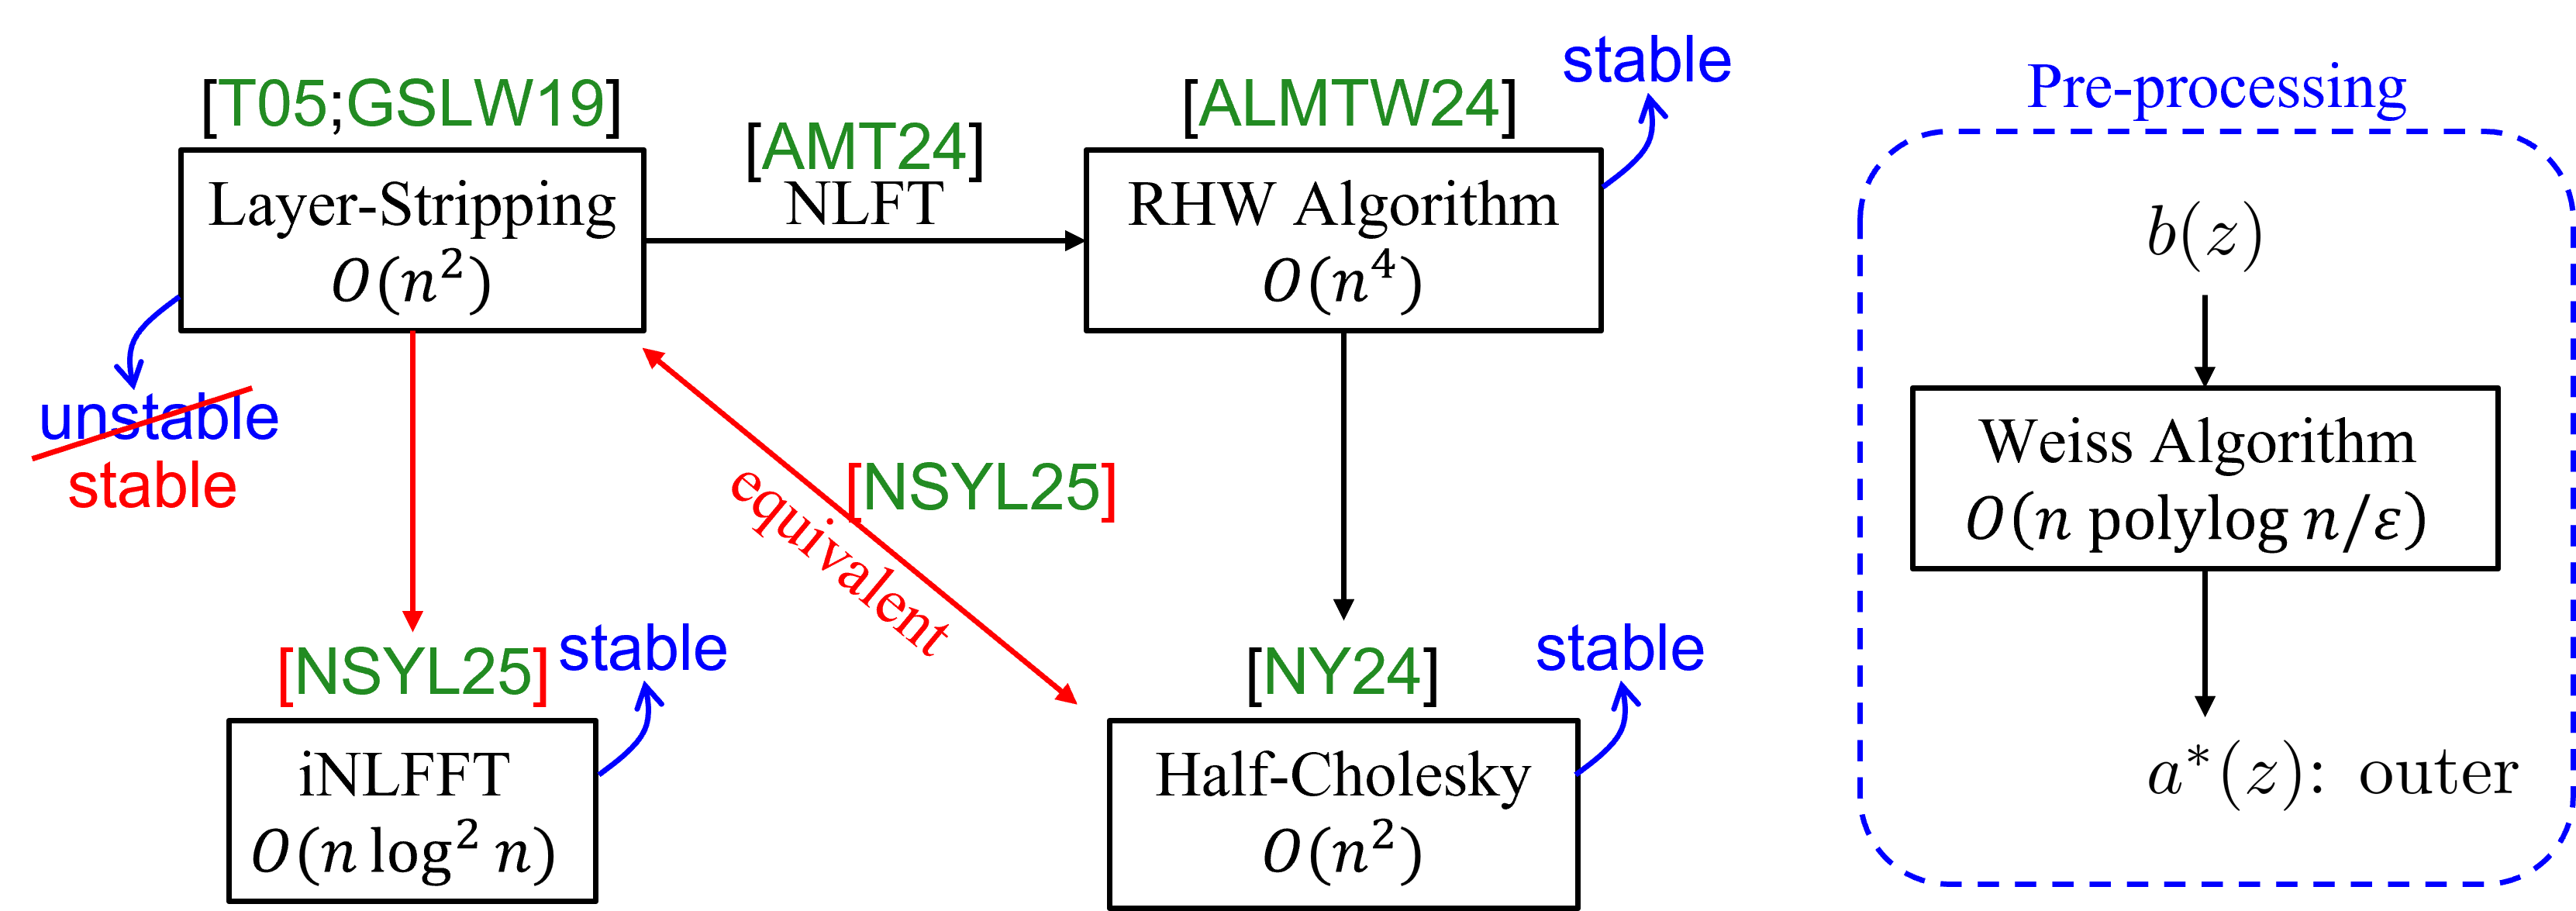
\includegraphics[width=1\linewidth]{figures/roadmap.png}
    \end{figure}
\end{frame}
% \begin{frame}{Code Implementation}
    
% \end{frame}

\begin{frame}{Future Directions}
    It is shown in \cite{Szego}, \cite{GQSP_NLFT}, and \cite{Lin2025} that the above methodology still holds in the case of infinite quantum signal processing, where the length of the phase sequence goes to infinity.
    
    Some future directions suggested includes:
    \begin{itemize}
        \item Is there a stable algorithm for \textit{non-outer} $a^*$?
        \item A stable algorithm for fully-coherent case: $\norm{b}_\infty=1$.
        \item Are all the behaviors of QSP in \cite{EnergyLandscpae} explained? Especially from the point of view of NLFT.
        \item M-QSP \cite{MQSP}: Is there any better choice of unitaries to span the whole space of multivariate functions?
        \item Is there a \textit{theoretical lower bound} to the complexity and bits required? Up to constants?
        \item ...
    \end{itemize}
\end{frame}